
\input{macrospresent}
\documentclass{beamer}

\newtheorem{examplee}{Ejemplo}
\usepackage{tikz-cd}
\usepackage{svg}
\usepackage{ragged2e}
\usepackage{amsmath}
\usepackage{tikz} % Diagramas conmutativos.
\usepackage{multicol}
\mode<presentation> {
  %%% Selección de estilo
  % The Beamer class comes with a number of default slide themes
  % which change the colors and layouts of slides. Below this is a list
  % of all the themes, uncomment each in turn to see what they look like.

  %\usetheme{default}
  %\usetheme{AnnArbor}
  %\usetheme{Antibes}
  %\usetheme{Bergen}
  %\usetheme{Berkeley}
  %\usetheme{Berlin}
  %\usetheme{Boadilla}
  %\usetheme{CambridgeUS}
  %\usetheme{Copenhagen}
  %\usetheme{Darmstadt}
  %\usetheme{Dresden}
  \usetheme{Frankfurt}
  %\usetheme{Goettingen}
  %\usetheme{Hannover}
  %\usetheme{Ilmenau}
  %\usetheme{JuanLesPins}
  %\usetheme{Luebeck}
  %\usetheme{Madrid}
  %\usetheme{Malmoe}
  %\usetheme{Marburg}
  %\usetheme{Montpellier}
  %\usetheme{PaloAlto}
  %\usetheme{Pittsburgh}
  %\usetheme{Rochester}
  %\usetheme{Singapore}
  %\usetheme{Szeged}
  %\usetheme{Warsaw}

\newenvironment{ejemplo2}[3]{%
  \setbeamercolor{block body}{#2}
  \setbeamercolor{block title}{#3}
  \begin{block}{#1}}{\end{block}}
  


 \setbeamercolor{ejemplo2}{parent=structure,fg=yellow,bg=cyan}
 
  %% Selección de color
  % As well as themes, the Beamer class has a number of color themes
  % for any slide theme. Uncomment each of these in turn to see how it
  % changes the colors of your current slide theme.

  %\usecolortheme{albatross}
  %\usecolortheme{beaver}
  %\usecolortheme{beetle}
  %\usecolortheme{crane}
  %\usecolortheme{dolphin}
  %\usecolortheme{dove}
  %\usecolortheme{fly}
  %\usecolortheme{lily}
  %\usecolortheme{orchid}
  %\usecolortheme{rose}
  %\usecolortheme{seagull}
  %\usecolortheme{seahorse}
  %\usecolortheme{whale}
  %\usecolortheme{wolverine}

  %% Configuración del pie de línea
  %\setbeamertemplate{footline} % To remove the footer line in all slides uncomment this line
  %\setbeamertemplate{footline}[page number] % To replace the footer line in all slides with a simple slide count uncomment this line
  \setbeamertemplate{navigation symbols}{} % To remove the navigation symbols from the bottom of all slides uncomment this line
}
\setbeamertemplate{footline}[frame number]

%% Fuentes de tamaño arbitrario
\usepackage{lmodern}
\usepackage{graphics,tikz}
\usetikzlibrary{automata, positioning, arrows, fit, shapes}
%% Gráficos
\usepackage{graphicx} % Allows including images
\usepackage{booktabs} % Allows the use of \toprule, \midrule and \bottomrule in tables

%%% Castellano.
% noquoting: Permite uso de comillas no españolas.
% lcroman: Permite la enumeración con numerales romanos en minúscula.
% fontenc: Usa la fuente completa para que pueda copiarse correctamente del pdf.

\usepackage[spanish,es-noquoting,es-lcroman,es-tabla]{babel}
\usepackage[utf8]{inputenc}
\usepackage[T1]{fontenc}
\usepackage[linesnumbered, onelanguage]{algorithm2e}
\usepackage{tabularx}
\usepackage{listings}
\selectlanguage{spanish}
\definecolor{Maroon}{cmyk}{0, 0.87, 0.88, 0.1}
\definecolor{teal}{rgb}{0.0, 0.45, 0.45}
\newcommand{\R}{\mathbb{R}}
\newcommand{\M}{\mathcal{M}}
\newcommand{\I}{\mathcal{I}}

\renewcommand\L{\mathcal{L}}
\newcommand{\G}{\mathcal{G}}
\newcommand\m[1]{\mathcal{#1}}
%\setbeamertemplate{footline}[frame number]
%\setbeamertemplate{footline}[split theme]
%----------------------------------------------------------------------------------------
%	TÍTULO
%----------------------------------------------------------------------------------------

\title[Algoritmos FCA]{Estudio experimental de algoritmos de cálculo de retículos en Análisis Formal de Conceptos} % The short title appears at the bottom of every slide, the full title is only on the title page

\author{Miguel Ángel Cantarero López} % Your name
\institute[UGR] % Your institution as it will appear on the bottom of every slide, may be shorthand to save space
{
  Universidad de Granada \\ % Your institution for the title page
  \medskip
  \textit{Doble grado en Ingeniería Informática y Matemáticas} % Your email address
}

\date{2 de diciembre de $2022$} % Date, can be changed to a custom date


\AtBeginSection[]{
	\begin{frame}
		\vfill
		\centering
		\begin{beamercolorbox}[sep=8pt,center,shadow=true,rounded=true]{title}
			\usebeamerfont{title}\insertsectionhead\par%
		\end{beamercolorbox}
		\vfill
	\end{frame}
}


\begin{document}

%% Diapositiva de título.
\frame[plain]{
\titlepage % Print the title page as the first slide
\small{\textit{Trabajo tutorizado por Nicolás Marín Ruiz y Daniel Sánchez Fernández}}
}

%% Diapositiva de contenidos.
% Throughout your presentation, if you choose to use \section{} and \subsection{} commands, 
% these will automatically be printed on this slide as an overview of your presentation

\frame[plain]{
  \frametitle{Contenidos} % Table of contents slide, comment this block out to remove it
  \tableofcontents
}


%----------------------------------------------------------------------------------------
%	PRESENTACIÓN
%----------------------------------------------------------------------------------------

%------------------------------------------------
\section{Introducción} 


\begin{frame}{Introducción}
\textit{El FCA es un campo de la matemática aplicada que formaliza matemáticamente el significado de la palabra ``concepto''.}
\vfill
\pause
\setbeamertemplate{items}[triangle]
\begin{itemize}
    \item \textbf{[1977]:} Retículos matemáticos desde un punto de vista computacional.
    \vspace{2mm}
    \pause
    \item \textbf{[1981]:} Rudolf Wille formaliza las ideas anteriores y crea el FCA.
    \vspace{2mm}
    \pause
    \item \textbf{[1999]:} Se publica el libro de Formal Concept Analysis (Bernhard Ganter y Rudolf Wille).
    \vspace{2mm}
    \pause
    \item \textbf{[2002]:} S. Kuznetsov y S. Obiedkov publican un artículo comparativo de algoritmos.
    \vspace{2mm}
    \pause
    \item \textbf{[2004]:} Comienzan las ICFCA.
\end{itemize}

\vspace{5mm}



\end{frame}


\begin{frame}{Motivación}

  \begin{columns}
      \begin{column}{0.6\textwidth}
        \begin{center}
        \vspace{-25mm}
        \textbf{Contexto formal}
        \vspace{-5mm}
        \begin{table}[H]
        \resizebox{7.5cm}{!}{
        \begin{tabular}{c|c|c|c|c|c|}
        \cline{2-6}
                                                                 & \textbf{Cine} & \textbf{Ropa} & \textbf{Alimentación} & \textbf{Pantalla Gigante} & \textbf{Electrónica} \\ \hline
        \multicolumn{1}{|c|}{\textbf{Nevada}}   &               & x            & x                    &                           & x                   \\ \hline
        \multicolumn{1}{|c|}{\textbf{Neptuno}}  & x            & x            & x                    &                           &                      \\ \hline
        \multicolumn{1}{|c|}{\textbf{Serrallo}} & x            & x            & x                    & x                        &                      \\ \hline
        \end{tabular}
        }
        \end{table}
        
        \vspace{15mm}
        \pause
        \textbf{Conceptos formales}
        \begin{itemize}
            \item \tiny(\{Nevada\},\{Ropa, Alimentación, Electrónica\})
            \item \tiny(\{Neptuno, Serrallo\},\{Cine,Ropa,Alimentación\})
        \end{itemize}
        \end{center}
      \end{column}
       \hspace{3mm}
       \pause
      \begin{column}{0.4\textwidth}  %%<--- here
        \begin{center}
            \begin{figure}[H]
            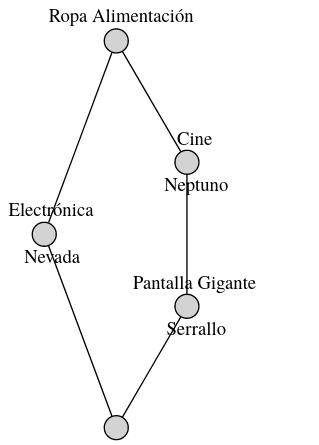
\includegraphics[scale=0.38]{images/grafo-comerciales.png}
            %\caption{Retículo de conceptos}.
            \end{figure}
            \textbf{Retículo de conceptos}
        \end{center}
      \end{column}
    \end{columns}
\end{frame}
  
  \begin{frame}{Objetivos}
      \begin{itemize}
          \item Comprender y explicar la Teoría del Análisis Formal de Conceptos.
          \vspace{4mm}
          \item Recopilar los algoritmos más importantes que existen en la literatura.
          \vspace{4mm}
          \item Implementar los algoritmos y analizar su desempeño mediante una experimentación equitativa.
          \vspace{4mm}
          \item Publicar la experimentación para que sea reproducible.
      \end{itemize}
  \end{frame}



\section{Teoría del Análisis Formal de Conceptos}
\begin{frame}{Contexto formal}
    \begin{block}{Definición (Contexto formal)} 
    \justifying
    Un contexto formal $\mathbb{K}:=(\G,\M,\I)$ está compuesto por un conjunto $\G$, cuyos elementos se llaman objetos, un conjunto $\M$, cuyos elementos se llaman atributos, y una relación binaria $\I \subseteq \G \times \M$. 
    \iffalse 
    Llamaremos a $\I$ la relación de incidencia y leeremos $(g,m) \in \I$ como ``el objeto $g$ tiene el atributo $m$''. 
    \fi
    \end{block}
  
     \vspace{6mm}
     \pause

      El contexto formal se traduce en la práctica a una tabla cruzada.
\end{frame}

\begin{frame}{Contexto formal}
    
        \begin{table}[H]
        \resizebox{\columnwidth}{!}{
        \begin{tabular}{c|c|c|c|c|c|}
        \cline{2-6}
                                                                 & \textbf{Cine} & \textbf{Ropa} & \textbf{Alimentación} & \textbf{Pantalla Gigante} & \textbf{Electrónica} \\ \hline
        \multicolumn{1}{|c|}{\textbf{Nevada}}   &               & x            & x                    &                           & x                   \\ \hline
        \multicolumn{1}{|c|}{\textbf{Neptuno}}  & x            & x            & x                    &                           &                      \\ \hline
        \multicolumn{1}{|c|}{\textbf{Serrallo}} & x            & x            & x                    & x                        &                      \\ \hline
        \end{tabular}
        }
        \end{table}
        \setbeamercolor{block title}{bg=green!30!black,fg=white}
        \begin{block}{Ejemplo 1}
         $$\G=\{\text{Nevada, Neptuno, Serrallo}\}.$$
         $$\M=\{\text{Cine, Ropa, Alimentación, Pantalla Gigante, Electrónica}\}.$$
         $\{$\begin{small}$\text{(Nevada, Ropa), (Nevada, Alimentación), (Nevada, Electrónica),}$\linebreak $\text{(Neptuno, Cine), (Neptuno, Ropa), (Neptuno, Alimentación), (Serrallo, }$ \linebreak $\text{ Cine), (Serrallo, Ropa), (Serrallo, Alimentación), (Serrallo, Pantalla)}\}$\end{small}
        \end{block}

\end{frame}

  \begin{frame}{Operadores de derivación}
    \begin{block}{Definición (Operador de derivación para objetos) }
    $\text{Sea } A\subseteq \G \ , \  A' := \{m \in \M \ | \ g \I m \ \ \forall g \in A\} \ , \ \{\emptyset\}'=\M$
    \end{block}
    
    \begin{block}{Definición (Operador de derivación para atributos) }
    $ \text{Sea } B\subseteq \M \ , \   B':= \{g \in \G \ |\  g \I m \ \ \forall m \in B\} \ , \ \{\emptyset\}'=\G
    $
    \end{block}
    \pause
        \vspace{-1mm}
        \begin{table}[H]
        \resizebox{9.6cm}{!}{
        \begin{tabular}{c|c|c|c|c|c|}
        \cline{2-6}
                                                                 & \textbf{Cine} & \textbf{Ropa} & \textbf{Alimentación} & \textbf{Pantalla Gigante} & \textbf{Electrónica} \\ \hline
        \multicolumn{1}{|c|}{\textbf{Nevada}}   &               & x            & x                    &                           & x                   \\ \hline
        \multicolumn{1}{|c|}{\textbf{Neptuno}}  & x            & x            & x                    &                           &                      \\ \hline
        \multicolumn{1}{|c|}{\textbf{Serrallo}} & x            & x            & x                    & x                        &                      \\ \hline
        \end{tabular}
        }
        \end{table}
        \vspace{-3mm}
        \setbeamercolor{block title}{bg=green!30!black,fg=white}
        \begin{block}{Ejemplo 2}
          $$\{\text{Neptuno}\}'=\{\text{Cine, Ropa, Alimentación}\}$$
          $$\{\text{Ropa, Electrónica}\}'=\{\text{Nevada}\}$$
        \end{block}
        
        \end{frame}
        
\iffalse
\begin{frame}{Operadores dobles de derivación}
        \vspace{-3mm}
        \begin{table}[H]
        \resizebox{\columnwidth}{!}{
        \begin{tabular}{c|c|c|c|c|c|}
        \cline{2-6}
                                                                 & \textbf{Cine} & \textbf{Ropa} & \textbf{Alimentación} & \textbf{Pantalla Gigante} & \textbf{Electrónica} \\ \hline
        \multicolumn{1}{|c|}{\textbf{Nevada}}   &               & x            & x                    &                           & x                   \\ \hline
        \multicolumn{1}{|c|}{\textbf{Neptuno}}  & x            & x            & x                    &                           &                      \\ \hline
        \multicolumn{1}{|c|}{\textbf{Serrallo}} & x            & x            & x                    & x                        &                      \\ \hline
        \end{tabular}
        }
        \end{table}
        
        \setbeamercolor{block title}{bg=green!30!black,fg=white}
        \begin{block}{Ejemplo 3}
        \vspace{-5mm}
        $$\{\text{Neptuno}\}''=\{\text{Cine, Ropa, Alimentación}\}'=\{\text{Neptuno, Serrallo}\}$$
        \vspace{-6mm}
         \begin{small}
          $$\{\text{Ropa, Electrónica}\}''=\{\text{Nevada}\}'=\{\text{Ropa, Alimentación, Electrónica}\}$$
        \end{small}
        \end{block}
        \pause
        \setbeamercolor{block title}{bg=blue!55!black,fg=white}
        \begin{block}{Definición (Operadores dobles de derivación)}
        $(\cdot )'':2^{|\G|} \to 2^{|\G|}$\linebreak
        $(\cdot )'': 2^{|\M|} \to 2^{|\M|} $
        \end{block}
        

        
        
  \end{frame}
  \fi
    \begin{frame}{Concepto formal}
      \begin{block}{Definición (Concepto formal)} 
      \justifying
      Un concepto formal de un contexto formal $\mathbb{K}:=(\G,\M,\I)$ se define como una pareja $(A,B) \subseteq \I$ con $A\subseteq \G$, $B\subseteq \M$, que cumple $A'=B$ y $B'=A$.
      \end{block}
      \pause
      \setbeamercolor{block title}{bg=green!30!black,fg=white}
      \begin{block}{Ejemplo 4 }
        $$(\{\text{Neptuno,Serrallo}\},\{\text{Cine,Ropa, Alimentación}\})$$
        %$$(\{\text{Nevada,Neptuno, Serrallo}\},\{\text{Ropa, Alimentación}\})$$
      \end{block}
       
       \begin{table}[H]
        \resizebox{\columnwidth}{!}{
        \begin{tabular}{c|c|c|c|c|c|}
        \cline{2-6}
                                                                 & \textbf{Cine} & \textbf{Ropa} & \textbf{Alimentación} & \textbf{Pantalla Gigante} & \textbf{Electrónica} \\ \hline
        \multicolumn{1}{|c|}{\textbf{Nevada}}   &               & x            & x                    &                           & x                   \\ \hline
        \multicolumn{1}{|c|}{\textbf{Neptuno}}  & {\color{teal}\textbf{x}}              & {\color{teal}\textbf{x}}              & {\color{teal}\textbf{x}}                      &                           &                      \\ \hline
        \multicolumn{1}{|c|}{\textbf{Serrallo}} & {\color{teal}\textbf{x}}            & {\color{teal}\textbf{x}}              & {\color{teal}
        \textbf{x}}                      & x                        &                      \\ \hline
        \end{tabular}
        }
        \end{table}

  \end{frame}


  \begin{frame}{Orden y Retículo de conceptos}
      \setbeamercolor{block title}{bg=blue!55!black,fg=white}
      \begin{block}{Definición (Relación de orden entre conceptos)}
      \justifying
        Sean $(A_1,B_1)$, $(A_2,B_2)$ conceptos formales, $(A_1,B_1)$ es un subconcepto de $(A_2,B_2)$ si $A_1 \subseteq A_2$  y  $B_2 \subseteq B_1$. Cuando esto ocurra escribiremos $(A_1,B_1) \leq (A_2,B_2)$.
      \end{block}
      \pause
      \begin{block}{Definición (Retículo de conceptos)}
      \justifying
      El conjunto de todos los conceptos formales de $(\G,\M,\I)$ ordenados por la anterior relación de orden ``$\leq$'' definida es un retículo de conceptos y se denota por 

    $$\underline{\mathfrak{B}}(\G,\M,\I):= (\mathfrak{B}(\G,\M,\I),\leq).$$
    \end{block}
\end{frame}
\begin{frame}{Retículo de conceptos}
    \setbeamercolor{block title}{bg=green!30!black,fg=white}

    \begin{columns}
    \begin{column}{0.75\textwidth}
    \begin{block}{Ejemplo 5}
    \begin{small}
      $\underline{\mathfrak{B}}(\G,\M,\I):=$\textbraceleft\linebreak(\{Nevada, Neptuno, Serrallo\}, \{Ropa, Alimentación\}),\linebreak (\{Nevada\}, \{Ropa, Alimentación, Electrónica\}),\linebreak \alert<3>{(\{Neptuno, Serrallo\}, \{Cine, Ropa, Alimentación\})},\linebreak (\{Serrallo\}, \{Cine, Ropa, Alimentación, Pantalla\}),\linebreak
      (\{$\emptyset$\},\{Cine, Ropa, Alimentación, Pantalla, Electrónica\})\linebreak
      \textbraceright 
      \end{small}
    \end{block}
    \pause
    \end{column}
    \hspace{-6mm}
    \begin{column}{0.25\textwidth}
             \begin{figure}[H]
            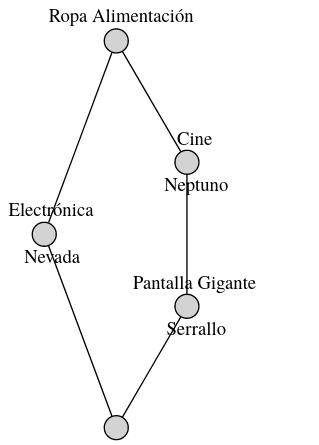
\includegraphics[scale=0.38]{images/grafo-comerciales.png}
            %\caption{Retículo de conceptos}.
    \end{figure}
    \end{column}

   \end{columns}
  \end{frame}

\begin{frame}{Teorema Básico del FCA }
      \setbeamercolor{block title}{bg=red!75!black,fg=white}
      \begin{block}{Teorema Básico de los Retículos de Conceptos (Parte I)}
      \justifying
      El retículo de conceptos de cualquier contexto $(\G,\M,\I)$ es un retículo completo. Para cualquier subconjunto arbitrario
    $$\{(A_t,B_t) | t\in T \} \subseteq\mathfrak{B}(\G,\M,\I),$$
    de conceptos formales, el ínfimo viene dado por
    
    \[
        \inf\{(A_{t}, B_{t})_{t \in T}\} = \bigwedge_{t\in T}(A_{t},B_{t})= (\bigcap_{t \in T}A_{t}, (\bigcup_{t \in T}B_{t})''),
    \]
    y el supremo viene dado por
    \[
        \sup\{(A_{t}, B_{t})_{t \in T}\} = \bigvee_{t\in T}(A_{t},B_{t})= ((\bigcup_{t \in T}A_{t})'', \bigcap_{t \in T}B_{t}).
    \]
    \end{block}
\end{frame}

    \begin{frame}{Teorema Básico del FCA }
    \setbeamercolor{block title}{bg=red!75!black,fg=white}
    \begin{block}{Teorema Básico de los Retículos de Conceptos (Parte II)}
    \justifying
    Un retículo completo $\underline{L}$ es isomorfo a $\underline{\mathfrak{B}}(\G,\M,\I)$ si y solo si existen funciones $\overline{\gamma}:\G \to L$ y $\overline{\mu}:\M \to L$ tales que $\overline{\gamma}(\G)$ es supremo-denso y $\overline{\mu}(\M)$ es ínfimo-denso en $\underline{L}$ y $$g \I m \Longleftrightarrow \overline{\gamma}(g) \leq \overline{\mu}(m), $$
    En particular $\underline{L} \cong \underline{\mathfrak{B}}(\G,\M,\I).$
    \end{block}
  \end{frame}

\begin{frame}{Aplicaciones}

\begin{itemize}
    \item Recuperación de información (buscadores).
    \vspace{4mm}
    \item Biología.
    \vspace{4mm}
    \item Diseño de software.
    \vspace{4mm}
    \item Análisis de datos (visualización, preprocesamiento, \dots ).
\end{itemize}
\end{frame}
\iffalse
\begin{frame}{Aplicaciones}
    \vspace{1mm}
    \begin{itemize}
        \item Recuperación de Información (Buscadores).
        \item Biología, análisis de datos, preprocesamiento, agrupamiento, visualización, $\dots$
    \end{itemize} 
    \vspace{-20mm}
    \pause
    \begin{columns}
    \begin{column}{0.5\textwidth}
    \vspace{15mm}
    \begin{table}[H]
    \resizebox{1.1\columnwidth}{!}{
    \begin{tabular}{c|c|c|c|c|}
    \cline{2-5}
                                              & \textbf{Álgebra} & \textbf{Ecuaciones} & {\color{Maroon} \textbf{Grupos}} & \textbf{Análisis} \\ \hline
    \multicolumn{1}{|c|}{\textbf{Documento1}} &                  &                     &                 & x                \\ \hline
    \multicolumn{1}{|c|}{\textbf{Documento2}} & x               &                     &                 & x                \\ \hline
    \multicolumn{1}{|c|}{\textbf{Documento3}} & x               &                     & x              &                   \\ \hline
    \multicolumn{1}{|c|}{\textbf{Documento4}} & x               & x                  & x              &                   \\ \hline
    \multicolumn{1}{|c|}{\textbf{Documento5}} & x               &                     & x              &                   \\ \hline
    \end{tabular}
    
    }
    \end{table}
    \vspace{-2mm}
    \centering
    Contexto de documentos, conceptos formales y retículo de conceptos asociado.
    \tiny{
    $$(\{\text{Documento2,Documento3,Documento5,Documento4}\},\{\text{Álgebra}\})$$
    {\color{Maroon} \textbf{(\{Documento3,Documento4,Documento5\},\{Álgebra,Grupos\})}}
    $$(\{\text{Documento4}\},\{\text{Álgebra,Grupos,Ecuaciones}\})$$
    }
    \end{column}
    \begin{column}{0.5\textwidth}
    \begin{center}
    \hspace{3mm}
            \begin{figure}[H]
            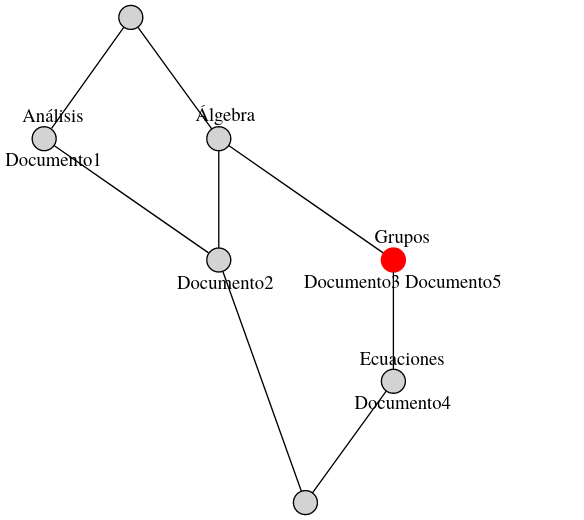
\includegraphics[scale=0.3]{images/documentos.png}
            \end{figure}
        \end{center}
    \end{column}
    \end{columns}

    %\begin{itemize}
    %    \item Biología, análisis de datos, preprocesamiento, agrupamiento, visualización,...
    %\end{itemize}
       
   \end{frame}
  \fi
\section{Algoritmos}
 
    \begin{frame}{Tipos}
    \justify
      \textbf{Objetivo:} Construir el retículo de conceptos a partir de un contexto formal según la aplicación que se le desee dar.
       \pause
        \begin{columns}[c]
          \begin{column}{0.35\textwidth}
            \begin{center}
                \setbeamercolor{block title}{bg=blue!75!black,fg=white}
                \begin{block}{\textbf{Por lotes (secuenciales)}}
                \begin{itemize}
                    \item NextClosure (Ganter).
                    \item Algoritmo de Lindig.
                    \item InClose.
                    \item Inherit-Concepts (Berry).
                    \item Algoritmo de Bordat.
                \end{itemize}
                \end{block}
            \end{center}
        \end{column}
        

          
        \begin{column}{0.29\textwidth}
            \setbeamertemplate{itemize item}{\color{red!70!black}$\bullet$}
            \setbeamercolor{block title}{bg=red!75!black,fg=white}
            \begin{center}
            \begin{block}{\textbf{Por lotes (paralelos)}}
                \begin{itemize}
                    \item MapReduce Ganter.
                    \item Algoritmo de Krajca.
                \end{itemize}
            \end{block}
            \end{center}
        \end{column}
        
        \pause
        \begin{column}{0.29\textwidth}
            \begin{center}
            \setbeamercolor{block title}{bg=blue!75!black,fg=white}
            \begin{block}{\textbf{Incrementales (secuenciales)}}
                \begin{itemize}
                    \item Norris.
                    \item Godin.
                    \item AddIntent.
                \end{itemize}
            \end{block}
            \end{center}
        \end{column}
          
      \end{columns}

  \end{frame}
  
\begin{frame}{Algoritmos}
    \begin{itemize}
        \item Tratan de evitar calcular varias veces el mismo concepto. 
    
        \item Heurísticas diferentes desarrolladas por sus autores.
    
     \item Basados en teoremas o propiedades desarrolladas por sus autores.
    \end{itemize}
    \pause

    \setbeamertemplate{itemize item}{\color{orange!90!black}$\bullet$}
    \setbeamercolor{block title}{bg=orange!95!black,fg=white}
     \begin{block}{\textbf{Algoritmo de Lindig}}
     \begin{itemize}

   \justifying
   \item Estrategia ``bottom-up''.
   
   \item Sea $(A,B)$ un concepto formal, 
   \begin{small}
   $$S=\{((A \cup \{g\})'',(A\cup \{g\})') | g \notin A\},$$ 
   \end{small}
   es el conjunto de todos los vecinos superiores de $(A,B)$.
   
   \end{itemize}
  \end{block}
    
    
    
  \end{frame}
  
  \begin{frame}{Implementación}
 
    \setbeamertemplate{itemize item}{\color{yellow!70!black}$\bullet$}
    \setbeamercolor{block title}{bg=yellow!80!black,fg=white}
    \begin{block}{\textbf{C++}:}
    \begin{itemize}
        \item $<$chrono$>$: \textit{steady\_clock::now()}
        \item $<$random$>$: \textit{uniform\_int\_distribution}
    \end{itemize}
    \end{block}
    \vspace{4mm}
    El contenido del trabajo se encuentra disponible en:
    \begin{center}
    {\color{Maroon} \url{https://github.com/miguecl97/TFG-AlgoritmosFCA}} , 
    \end{center}
    tanto datasets, retículos del resultado, pruebas de caja negra, \dots
  \end{frame}
\iffalse
\begin{frame}{Algoritmos por lotes}
    \setbeamertemplate{itemize item}{\color{orange!90!black}$\bullet$}
    \setbeamercolor{block title}{bg=orange!95!black,fg=white}

  \begin{block}{\textbf{NextClosure} (Algoritmo de Ganter)}
  \begin{itemize}
    \justifying

    \item Los operadores dobles de derivación forman un sistema de clausura para los conceptos.
  
    \item Si $(A,B)$ es un concepto, $A'=B$ y $B'=A$. Entonces:\linebreak
    \begin{small}
    $A''=(A')'=B'=A \ \text{y} \ B''=(B')'=A'=B$
    \end{small}
    \item Todos los $A$ que sean extensiones de conceptos son conjuntos cerrados. (Análogo para las intensiones).
    \end{itemize}
   \end{block}
   \pause
  \begin{block}{\textbf{Algoritmo de Lindig}}
  \begin{itemize}

   \justifying
   \item Estrategia ``bottom-up''.
   
   \item Sea $(A,B)$ un concepto formal, 
   \begin{small}
   $$S=\{((A \cup \{g\})'',(A\cup \{g\})') | g \notin A\},$$ 
   \end{small}
   es el conjunto de todos los vecinos superiores de $(A,B)$.
   
   \end{itemize}
  \end{block}
  
  \end{frame}
  
     \begin{frame}{Algoritmos por lotes}
     \setbeamertemplate{itemize item}{\color{orange!90!black}$\bullet$}
     \setbeamercolor{block title}{bg=orange!95!black,fg=white}
    
    \begin{block}{\textbf{Bordat}}
    \begin{itemize}
    \item Estrategia ``top-down''.
    
    \item Calcular los vecinos inferiores hasta completar el retículo.
    \end{itemize}
    \end{block}
    \pause
    \begin{block}{\textbf{InheritConcepts} (Algoritmo de Berry)}
    \begin{itemize}
    \item Emplea dos estructuras auxiliares para almacenar información sobre las relaciones entre los atributos.
    \end{itemize}
    \end{block}
    \pause
    \begin{block}{\textbf{InClose}}
    \begin{itemize}
    \item Calcula las extensiones incrementalmente, hasta que se termine o pode la rama.
      $A_{new}= A \cap \{j\}'$ , $\begin{cases} A_{new}=\emptyset,  \\
      \emptyset \neq A_{new} \subseteq A, \\
      A_{new} = A \Longrightarrow \text{Se poda la rama}.
      \end{cases}$
     \end{itemize}
     \end{block}
  \end{frame}
  
    \begin{frame}{Algoritmos incrementales}
    \setbeamertemplate{itemize item}{\color{orange!90!black}$\bullet$}
    \setbeamercolor{block title}{bg=orange!95!black,fg=white}

    \begin{block}{\textbf{Norris}}
    \begin{itemize}
        \item  Se recorre el árbol y se comprueba si el objeto añadir pertenece a los nodos o no. 
    \end{itemize}
    \end{block}
    \pause
    \begin{block}{\textbf{Godin}}
    \begin{itemize}
        \item  Se basa en la longitud de las extensiones para calcular a que nodo pertenece el objeto a añadir.
    \end{itemize}

    \end{block}
    \pause
    \begin{block}{\textbf{AddIntent}}
    \begin{itemize}
        \item  Se busca el concepto generador del objeto que se desea añadir. Añade el objeto a la extensión de los que están por encima y añade el atributo a la intensión de los que están por debajo.
    \end{itemize}

    \end{block}
  \end{frame}
  \fi
\iffalse
    \begin{frame}{Propiedades}
      \begin{table}[H]
\centering
\resizebox{\columnwidth}{!}{
\begin{tabular}{|l|c|c|c|c|c|c|c|c|}
\hline
Algoritmo                         & \textbf{p1} & \textbf{p2} & \textbf{p3} & \textbf{p4} & \textbf{p5} & \textbf{p6} & \textbf{p7} & \textbf{p8} \\ \hline
\textbf{NextClosure (Ganter)}   &             & x           & x           & x           &             & x           &             &             \\ \hline
\textbf{Lindig}                   &             & x           &             & x           & x           &             & x           & x           \\ \hline
\textbf{InClose}                  &             & x           & x           & x           &             & x           &             & x           \\ \hline
\textbf{Inherit-Concepts (Berry)} &             & x           &             &             & x           &             &             &             \\ \hline
\textbf{Bordat}                   &             & x           &             &             &             &             & x           &             \\ \hline
\textbf{Norris}                   & x           &             &             &             & x           &             &             & x           \\ \hline
\textbf{Godin}                    & x           &             &             &             & x           &             &             & x           \\ \hline
\textbf{AddIntent}                & x           &             &             &             & x           &             & x           & x           \\ \hline
\end{tabular}
}
\caption{p1 - incremental;
p2 - por lotes;
p3 - utiliza el orden léxico;
p4 - en cada paso selecciona un concepto actual;
p5 - utiliza  alguna estructura auxiliar;
p6 - emplea un test de canonicidad para evitar repetir cálculos;
p7 - calcula vecinos de los conceptos;
p8 - calcula las intersecciones de las intensiones que no son objetos y las intensiones de los objetos;}
\end{table}

\end{frame}
\fi

\section{Experimentación}


 \begin{frame}{Conjuntos de datos}


    \textbf{Valores:}
    \begin{itemize}
        \item Número de atributos: \textbf{$|\M|$} (lo fijaremos en \textbf{100}).
        \pause
        \item Número de objetos: \textbf{$|\G|$} (\textbf{variando} para cada ejecución de los experimentos).
        \pause
        \item Número medio de atributos que tiene cada objeto: \textbf{$|g'|$} \linebreak (\textbf{fijo} para cada experimento).
    \end{itemize}
    \vspace{10mm}
    \pause
        Los atributos que posee cada objeto se eligen generando números aleatorios siguiendo una distribución uniforme.

  \end{frame}
  
 \iffalse
  \begin{frame}{Software}
    \setbeamertemplate{itemize item}{\color{yellow!70!black}$\bullet$}
    \setbeamercolor{block title}{bg=yellow!80!black,fg=white}
    \begin{block}{\textbf{C++}:}
    \begin{itemize}
        \item $<$random$>$: \textit{uniform\_int\_distribution}
        \item $<$chrono$>$: \textit{steady\_clock::now()}
    \end{itemize}

    \end{block}
    \pause
    \begin{block}{\textbf{Python}:}
        \begin{itemize}
        \item pandas
        \item concepts
     \end{itemize}

    \end{block}
\end{frame}

\fi
  \iffalse
  \begin{frame}{Resultados (Conjuntos artificiales)}
      \begin{figure}[H]
      \centering
      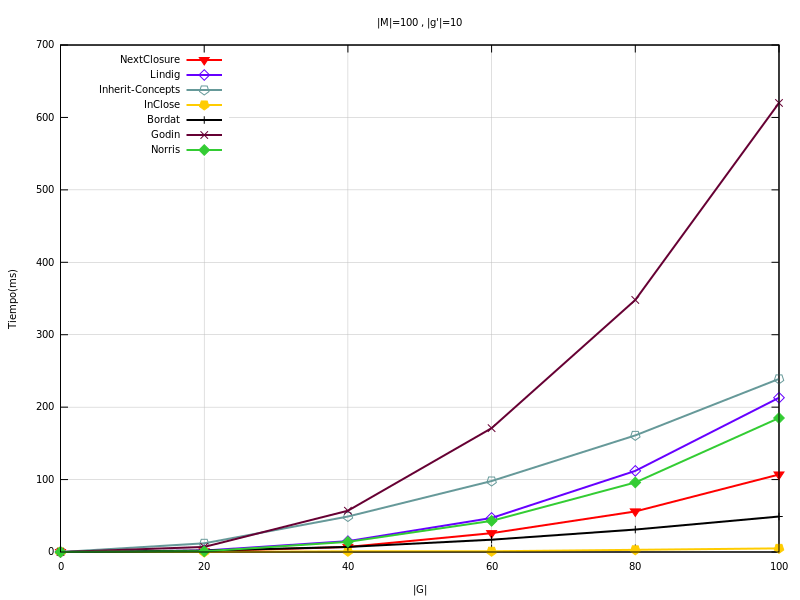
\includegraphics[scale=0.3]{images/M100g10G20100notadd.png}
      \caption{$|\M|=100$ , $|g'|=10$, $|\G|=\{20,40,60,80,100\}$}
     \end{figure}
  \end{frame}
  \fi
  
    \begin{frame}{Resultados (Conjuntos artificiales)}
      \begin{figure}[H]
      \centering
      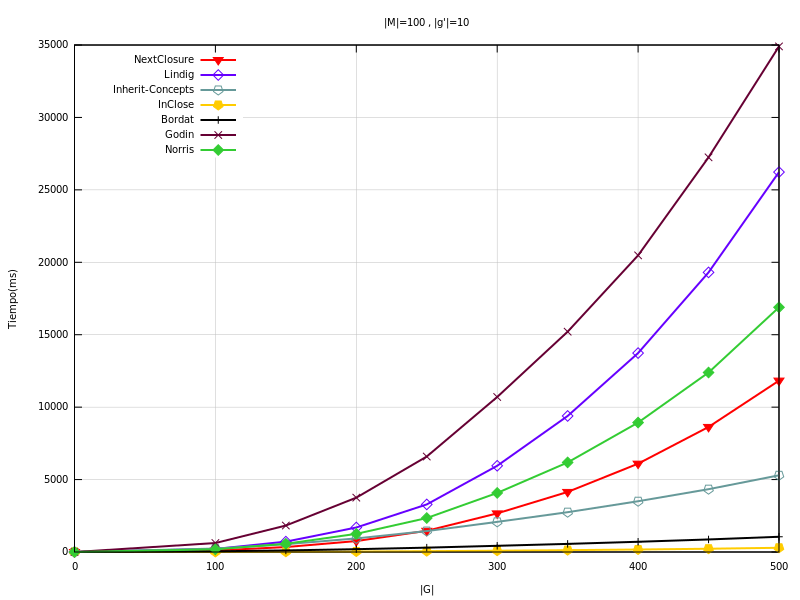
\includegraphics[scale=0.3]{images/M100g10G100500notadd.png}
      \caption{$|\M|=100$ , $|g'|=10$, $|\G|=\{100,200,300,400,500\}$}
     \end{figure}
  \end{frame}
  
       \begin{frame}{Resultados (Conjuntos artificiales)}
      \begin{figure}[H]
      \centering
      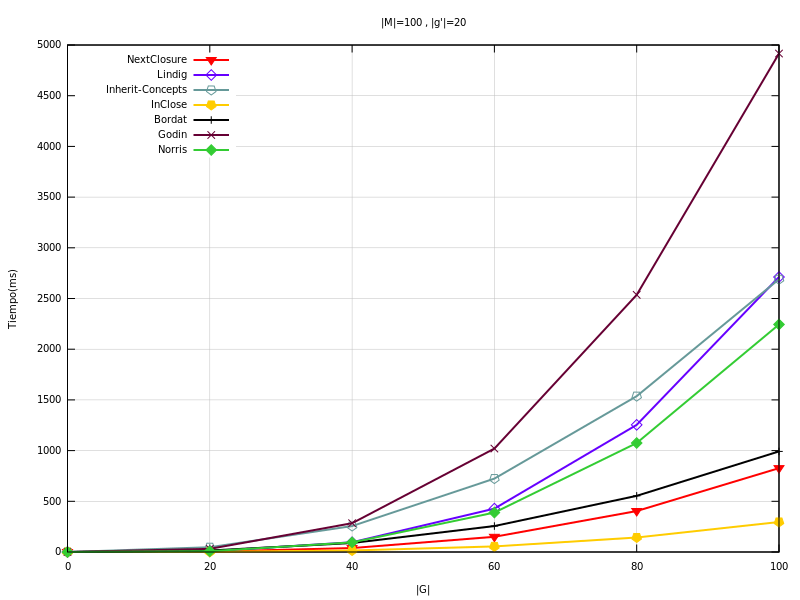
\includegraphics[scale=0.3]{images/M100g20G20100.png}
      \caption{$|\M|=100$ , $|g'|=20$, $|\G|=\{20,40,60,80,100\}$}
     \end{figure}
  \end{frame}
  
    \begin{frame}{Resultados (Conjuntos artificiales)}
      \begin{figure}[H]
      \centering
      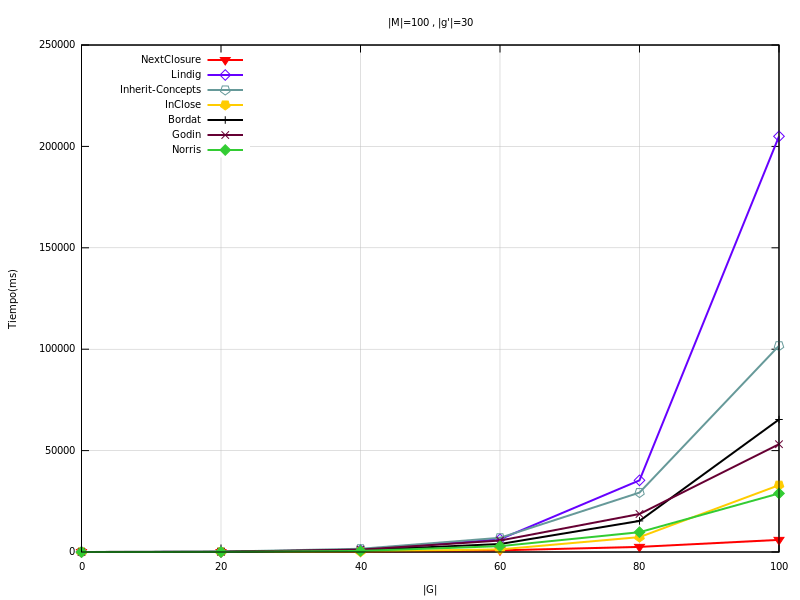
\includegraphics[scale=0.3]{images/M100g30G20100.png}
      \caption{$|\M|=100$ , $|g'|=30$, $|\G|=\{20,40,60,80,100\}$}
     \end{figure}
  \end{frame}
  
\begin{frame}{Resultados (Conjuntos artificiales)}
      \begin{figure}[H]
      \centering
      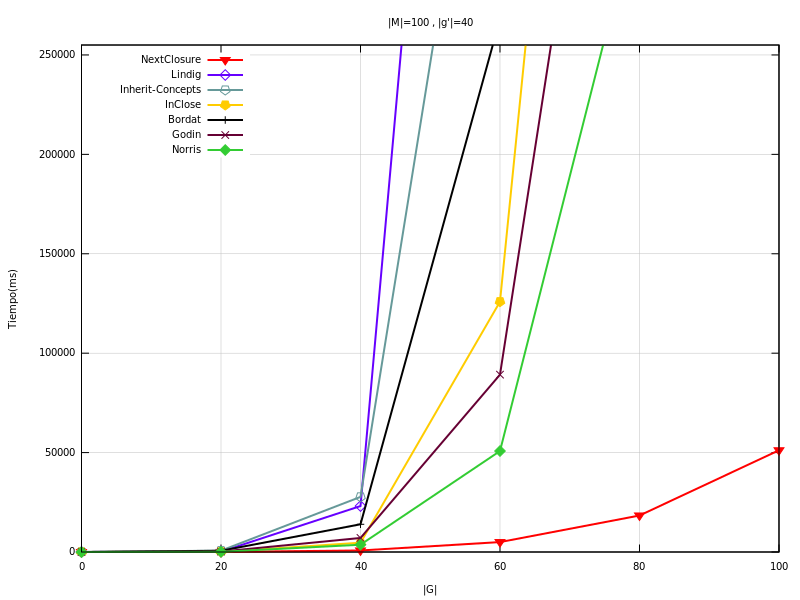
\includegraphics[scale=0.3]{images/M100g40G20100.png}
      \caption{$|\M|=100$ , $|g'|=40$, $|\G|=\{20,40,60,80,100\}$}
     \end{figure}
  \end{frame}
     \iffalse
     \begin{frame}{Resultados (Conjuntos de datos reales)}
      \textbf{BreastCancer.csv  ($|\M|=99$,$|g'|=10$,$|\G|=500$)}
      \begin{figure}[H]
        \centering
        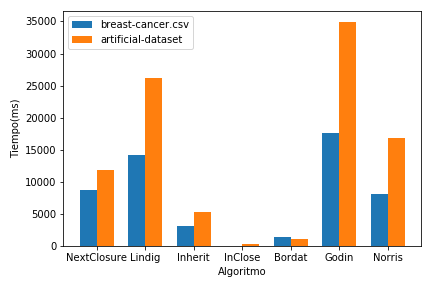
\includegraphics[scale=0.6]{images/comparative-breast.png}
      \end{figure}
  \end{frame}
  \fi
  
    \begin{frame}{Resultados (Conjuntos de datos reales)}
      \textbf{Sponges.csv ($|\M|=100$,$|g'|=29$,$|\G|=76$) }
      \begin{figure}[H]
      \centering
      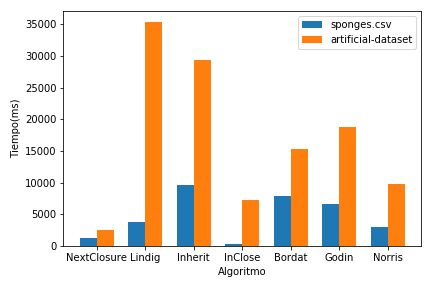
\includegraphics[scale=0.6]{images/comparative-sponges.png}
        \end{figure}
    \end{frame}
    
    \iffalse
    \begin{frame}{Distribuciones}
    \hspace{-7.mm}
      \minipage{0.5\textwidth}%
      \centering
      Artificial
      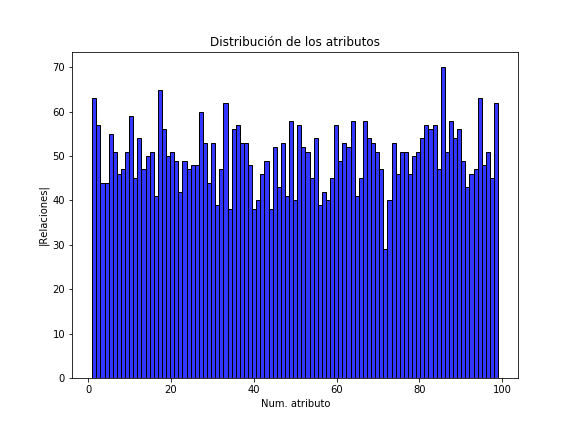
\includegraphics[scale=0.3]{images/distribution-artificialg10G500.png}
      \endminipage
      \hspace{3mm}
      \minipage{0.5\textwidth}%
      \centering
      Breast
      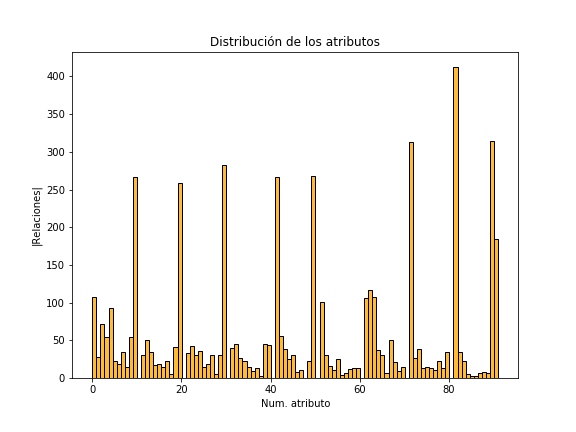
\includegraphics[scale=0.3]{images/distribution-breast.png}
      \endminipage

  \end{frame}
  \fi
      \begin{frame}{Distribuciones}
        \hspace{-7.mm}
      \minipage{0.5\textwidth}%
      \centering
      Artificial
      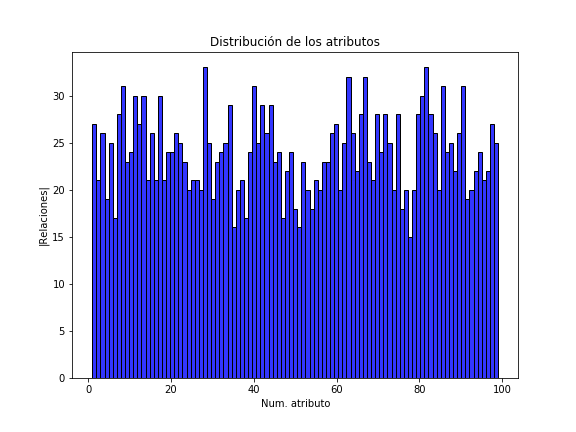
\includegraphics[scale=0.3]{images/distribution-artificialg30G80.png}
      \endminipage
      \hspace{3mm}
      \minipage{0.5\textwidth}%
      \centering
      Sponges.csv
      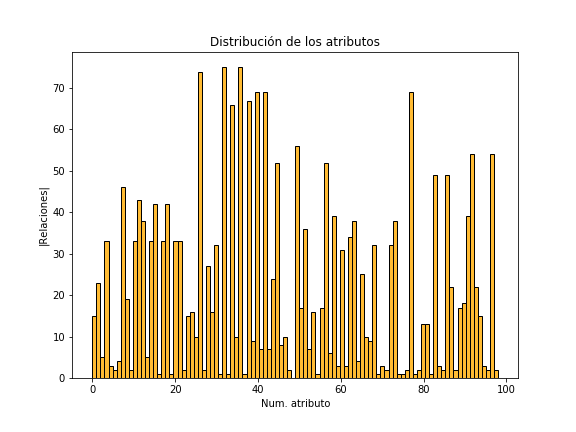
\includegraphics[scale=0.3]{images/distribution-sponges.png}
      \endminipage
  \end{frame}


\section{Conclusiones y vías futuras}

\begin{frame}{Conclusiones}

    \begin{itemize}
    \justifying
      \item Hemos obtenido una imagen del estado de los principales algoritmos que existen para el cálculo de retículos de conceptos.
      \vspace{2mm}
      \pause
      \item Ante conjuntos de datos cuyas relaciones de los atributos sigan una distribución uniforme y que tengan poca densidad, el algoritmo que menor tiempo de ejecución requiere es el InClose.
      \vspace{2mm}
      \item Si el conjunto de datos tiene una densidad elevada el algoritmo que mejor funciona es el NextClosure.
      \vspace{2mm}
      \item Si la distribución de los atributos en el conjunto de datos no sigue una distribución uniforme no podemos predecir el desempeño de los algoritmos con este estudio.
      \pause
      \vspace{2mm}
      \item Hemos visto una aplicación a los conocimientos que hemos aprendido durante el  grado de Matemáticas y del grado en Ingeniería Informática, que requiere de ambas competencias para su correcta comprensión y puesta en práctica.
    \end{itemize}
\end{frame}


\begin{frame}{Trabajo futuro}

\begin{itemize}
    \justifying
    \item Repetir la experimentación utilizando otra distribución de las relaciones de los atributos, no necesariamente uniforme, para así tener más casuísticas que permitan predecir el comportamiento de los algoritmos ante otros tipos de conjuntos de datos.
    \vspace{4mm}    
    \item Paralelizar los algoritmos que mejor rendimiento han tenido como el InClose o el NextClosure y comparar la mejora en tiempo de ejecución.
    \vspace{4mm}
    \item Realizar un análisis en profundidad de los algoritmos paralelos que existen en la literatura e incorporarlos al estudio.
    
\end{itemize}
\end{frame}

\appendix

\iffalse

\begin{frame}
\frametitle{Blocks of Highlighted Text}
\begin{block}{Block 1}
Lorem ipsum dolor sit amet, consectetur adipiscing elit. Integer lectus nisl, ultricies in feugiat rutrum, porttitor sit amet augue. Aliquam ut tortor mauris. Sed volutpat ante purus, quis accumsan dolor.
\end{block}
\end{frame}

%------------------------------------------------

\begin{frame}
\frametitle{Multiple Columns}
\begin{columns}[c] % The "c" option specifies centered vertical alignment while the "t" option is used for top vertical alignment

\column{.45\textwidth} % Left column and width
\textbf{Heading}
\begin{enumerate}
\item Statement
\item Explanation
\item Example
\end{enumerate}

\column{.5\textwidth} % Right column and width
Lorem ipsum dolor sit amet, consectetur adipiscing elit. Integer lectus nisl, ultricies in feugiat rutrum, porttitor sit amet augue. Aliquam ut tortor mauris. Sed volutpat ante purus, quis accumsan dolor.

\end{columns}
\end{frame}

\begin{frame}
\frametitle{Table}
\begin{table}
\begin{tabular}{l l l}
\toprule
\textbf{Treatments} & \textbf{Response 1} & \textbf{Response 2}\\
\midrule
Treatment 1 & 0.0003262 & 0.562 \\
Treatment 2 & 0.0015681 & 0.910 \\
Treatment 3 & 0.0009271 & 0.296 \\
\bottomrule
\end{tabular}
\caption{Table caption}
\end{table}
\end{frame}


%------------------------------------------------

\begin{frame}[fragile] % Need to use the fragile option when verbatim is used in the slide
\frametitle{Verbatim}
\begin{example}[Theorem Slide Code]
\begin{verbatim}
\begin{frame}
\frametitle{Theorem}
\begin{theorem}[Mass--energy equivalence]
$E = mc^2$
\end{theorem}
\end{frame}\end{verbatim}
\end{example}
\end{frame}


\begin{frame}
\frametitle{Figure}
Uncomment the code on this slide to include your own image from the same directory as the template .TeX file.
%\begin{figure}
%\includegraphics[width=0.8\linewidth]{test}
%\end{figure}
\end{frame}
\fi


















\iffalse
%------------------------------------------------

\begin{frame}[fragile] % Need to use the fragile option when verbatim is used in the slide
\frametitle{Citation}
An example of the \verb|\cite| command to cite within the presentation:\\~

This statement requires citation \cite{p1}.
\end{frame}

%------------------------------------------------
\fi




%% Bibliografía
\iffalse
\frame[plain]{
\frametitle{Bibliografía fundamental}
\footnotesize{

  \begin{thebibliography}{99} % Beamer does not support BibTeX so references must be inserted manually as below
  
      \bibitem[abstractmorado, 2017]{p1}
        Bernhard Ganter and Rudolf Wille (1999)
      \newblock Formal Concept Analysis
      \newblock \emph{Springer Berlin Heidelberg}
      
    \bibitem[abstract, 2002]{p1} Davey B. A. and Priestley  H. A. (2002)
      \newblock Introduction to Lattices and Order
      \newblock \emph{Cambridge University Press}
      
    \bibitem[green, 2006]{p1}
      Sergei Kuznetsov and Sergei Obiedkov (2002)
      \newblock Comparing performance of algorithms for generating concept lattices
      \newblock \emph{J. Exp. Theor. Arificial Intelligence}
      
     
    \bibitem[kmill, 2016]{p1}
        Olga Prokasheva, Alina Onishchenko, and Sergey Gurov (2013)
        \newblock Classification Methods Based on Formal Concept Analysis
        \newblock \emph{Faculty of Computational Mathematics and Cybernetics, Moscow State University}

      
      
  \end{thebibliography}
}

}
\fi

%------------------------------------------------

\frame[plain]{
\Huge{\centerline{Gracias por su atención.}}
}

%unsolvable WP https://eprint.iacr.org/2014/528.pdf

%----------------------------------------------------------------------------------------

\frame[plain]{
\frametitle{Ejecución incremental}
        \begin{table}[H]
        \resizebox{\columnwidth}{!}{
        \begin{tabular}{l|l|l|l|l|}
        \hline
        \multicolumn{1}{|l|}{$|g'|$} & $|\G|$                                        & \textbf{NextClosure} & \textbf{Norris}   & \textbf{Godin}    \\ \hline
        \multicolumn{1}{|l|}{40}     & 60                                            & 4990        & 50786    & 89212,9  \\ \hline
        \multicolumn{1}{|l|}{40}     & 80                                            & 18359,5     & 327035,3 & 542232,6 \\ \hline
                                     & Tiempo(ms) en añadir 20 objetos (de 60 a 80): & 23349,5     & 327035,3 & 542232,6 \\ \cline{2-5} 
        \end{tabular}
        }
        \caption{Tabla comparativa de tiempos de ejecución en ms para $|\M|=100$, que tardaría cada algoritmo en añadir 20 objetos al retículo.}
        \end{table}
        
        \begin{table}[H]
            \resizebox{\columnwidth}{!}{
            \begin{tabular}{|l|l|l|l|l|l|}
            \hline
            $|g'|$ & $|\G|$             & \textbf{NextClosure} & \textbf{Norris} & \textbf{NextClosure (incrementalmente)} & \textbf{Norris (incrementalmente)} \\ \hline
            10     & 20                 & 1           & 1,8    & 1                         & 1,8                  \\ \hline
            10     & 40                 & 7,6         & 7,88   & 8,6                       & 7,88                 \\ \hline
            10     & 60                 & 26,7        & 43,88  & 35,3                      & 43,88                \\ \hline
            10     & 80                 & 56,2        & 95     & 91,5                      & 95                   \\ \hline
            10     & 100                & 107,1       & 185,1  & 198,6                     & 185,1                \\ \hline
                   & Tiempo total (ms): &             &        & 197,1                     & 185,1                \\ \hline
            \end{tabular}
            }
            \caption{Tabla comparativa de tiempos de ejecución para una ejecución incremental con $|\M|=100$ y $|g'|=10$.}
            
            \label{tab:incremen10}
        \end{table}

}

\frame[plain]{
\frametitle{Retículo de propiedades}
      \begin{figure}[H]
        \centering
        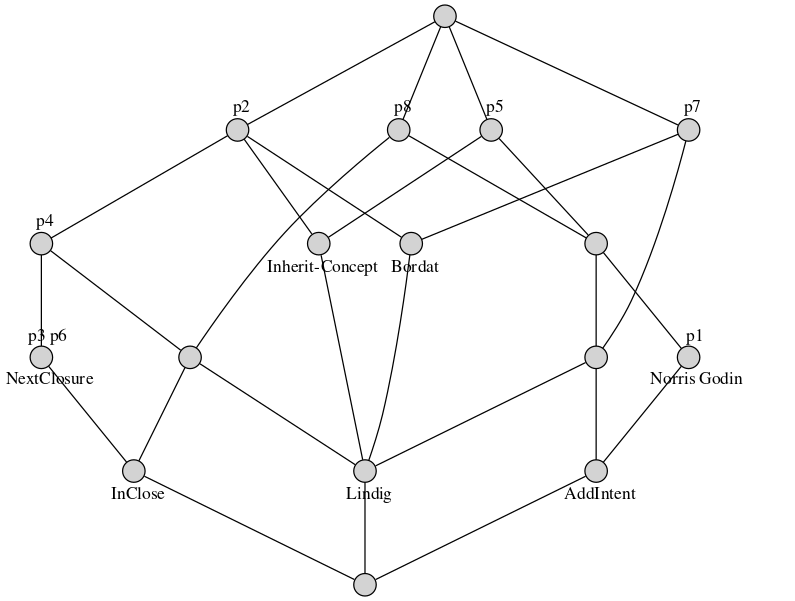
\includegraphics[scale=0.4]{images/PROPRET.png}
      \end{figure}
}


\frame[plain]{
\frametitle{Diferencia distribución atributos}
\begin{figure}[H]
\centering
\begin{minipage}{.4\textwidth}
  \centering
    \begin{table}[H]
    \begin{tabular}{|l|l|l|l|l|}
    \hline
       & a1 & a2 & a3 & a4 \\ \hline
    o1 & ~  & X  & X  & ~  \\ \hline
    o2 & X  & ~  & X  & ~  \\ \hline
    o3 & ~  & X  & ~  & X  \\ \hline
    \end{tabular}
    \end{table}
\end{minipage}%
\begin{minipage}{.6\textwidth}
  \centering
\begin{itemize}
    \item Concepto 1: (\{\}, \{a1, a2, a3, a4\}) 
    \item Concepto 2: (\{o1\}, \{a2, a3\}) 
    \item Concepto 3: (\{o2\}, \{a1, a3\}) 
    \item Concepto 4: (\{o3\}, \{a2, a4\}) 
    \item Concepto 5: (\{o1, o2\}, \{a3\}) 
    \item Concepto 6: (\{o1, o3\}, \{a2\}) 
    \item Concepto 7: (\{o1, o2, o3\}, \{\}) 
\end{itemize}
\end{minipage}
%\caption{Ejemplo de un contexto con $|\M|=4$, $|g'|=2$ y $|\G|=3$ , con una distribución que siguen los atributos que es uniforme junto con la lista de conceptos de su retículo. }
  %\label{fig:test1}
\end{figure}
\vspace{10mm}
\begin{figure}[H]
\centering
\begin{minipage}{.4\textwidth}
  \centering
    \begin{table}[H]
    \begin{tabular}{|l|l|l|l|l|}
    \hline
       & a1 & a2 & a3 & a4 \\ \hline
    o1 & X  & X  & ~  & ~ \\ \hline
    o2 & X  & ~  & ~  & ~  \\ \hline
    o3 & X  & ~  & X  & X  \\ \hline
    \end{tabular}
    \end{table}
\end{minipage}%
\begin{minipage}{.6\textwidth}
  \centering
\begin{itemize}
    \item Concepto 1: (\{\}, \{a1, a2, a3, a4\}) 
    \item Concepto 2: (\{o1\}, \{a1, a2\}) 
    \item Concepto 3: (\{o3\}, \{a1, a3, a4\}) 
    \item Concepto 4: (\{o1, o2, o3\}, \{a1\}) 
\end{itemize}
\end{minipage}
\end{figure}
}

\frame[plain]{
\frametitle{Resultados (Conjuntos de datos reales)}
      \begin{figure}[H]
      \centering
      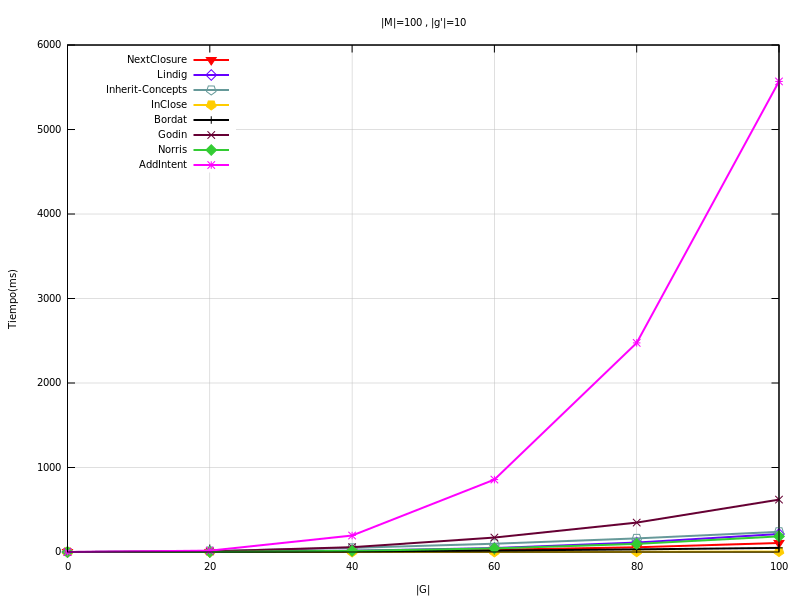
\includegraphics[scale=0.3]{images/M100g10G20100.png}
    \end{figure}
}

\frame[plain]{
\frametitle{Aplicaciones}
    \vspace{1mm}
    \begin{itemize}
        \item Recuperación de Información (Buscadores).
        \item Biología, análisis de datos, preprocesamiento, agrupamiento, visualización, $\dots$
    \end{itemize} 
    \vspace{-20mm}
    \pause
    \begin{columns}
    \begin{column}{0.5\textwidth}
    \vspace{15mm}
    \begin{table}[H]
    \resizebox{1.1\columnwidth}{!}{
    \begin{tabular}{c|c|c|c|c|}
    \cline{2-5}
                                              & \textbf{Álgebra} & \textbf{Ecuaciones} & {\color{Maroon} \textbf{Grupos}} & \textbf{Análisis} \\ \hline
    \multicolumn{1}{|c|}{\textbf{Documento1}} &                  &                     &                 & x                \\ \hline
    \multicolumn{1}{|c|}{\textbf{Documento2}} & x               &                     &                 & x                \\ \hline
    \multicolumn{1}{|c|}{\textbf{Documento3}} & x               &                     & x              &                   \\ \hline
    \multicolumn{1}{|c|}{\textbf{Documento4}} & x               & x                  & x              &                   \\ \hline
    \multicolumn{1}{|c|}{\textbf{Documento5}} & x               &                     & x              &                   \\ \hline
    \end{tabular}
    
    }
    \end{table}
    \vspace{-2mm}
    \centering
    Contexto de documentos, conceptos formales y retículo de conceptos asociado.
    \tiny{
    $$(\{\text{Documento2,Documento3,Documento5,Documento4}\},\{\text{Álgebra}\})$$
    {\color{Maroon} \textbf{(\{Documento3,Documento4,Documento5\},\{Álgebra,Grupos\})}}
    $$(\{\text{Documento4}\},\{\text{Álgebra,Grupos,Ecuaciones}\})$$
    }
    \end{column}
    \begin{column}{0.5\textwidth}
    \begin{center}
    \hspace{3mm}
            \begin{figure}[H]
            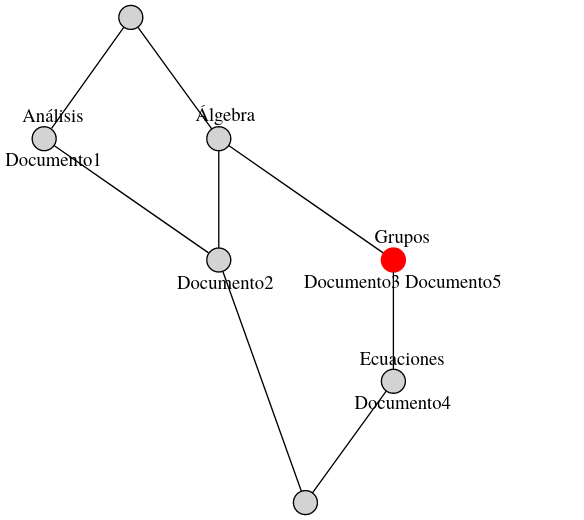
\includegraphics[scale=0.3]{images/documentos.png}
            \end{figure}
        \end{center}
    \end{column}
    \end{columns}

    %\begin{itemize}
    %    \item Biología, análisis de datos, preprocesamiento, agrupamiento, visualización,...
    %\end{itemize}
       
}
    
\end{document} 





